\chapter{Results}
%%%%%%%%%%%%%%%%%%%%%%%%%%%%%%%%%%%%%%%%%%%%%%%%%%%%%%%%%%%%%%%%%%
In this section we will first present the results from our case study and afterward will report on the results that we have got from the survey.

%%%%%%%%%%%%%%%%%%%%%%%%%%%%%%%%%%%%%%%%%%%%%%%%%%%%%%%%%%%%%%%
\section{The case study}
%%%%%%%%%%%%%%%%%%%%%%%%%%%%%%%%%%%%%%%%%%%%%%%%%%%%%%%%%%%%%%%

After running a word frequency query to gain some general insight about the data, we came to the result that are presented in Figure \ref{fig:wordcloud}, here the results are limited to the first 100 most frequent words. As we see here the word “works”, after omitting irrelevant words like pronouns, etc. is the most used word in backend, frontend, operations and help forums with a frequency of 2770. Smiling is the second word here which is repeated for more than 1900 times and the reason is that smileys or emoji are shown in logs as “:smile:” or “:smiling\_face:”. A list of the first 10 most used words is presented in Table \ref{table:word}.

\begin{figure}[hbt!]
\centering
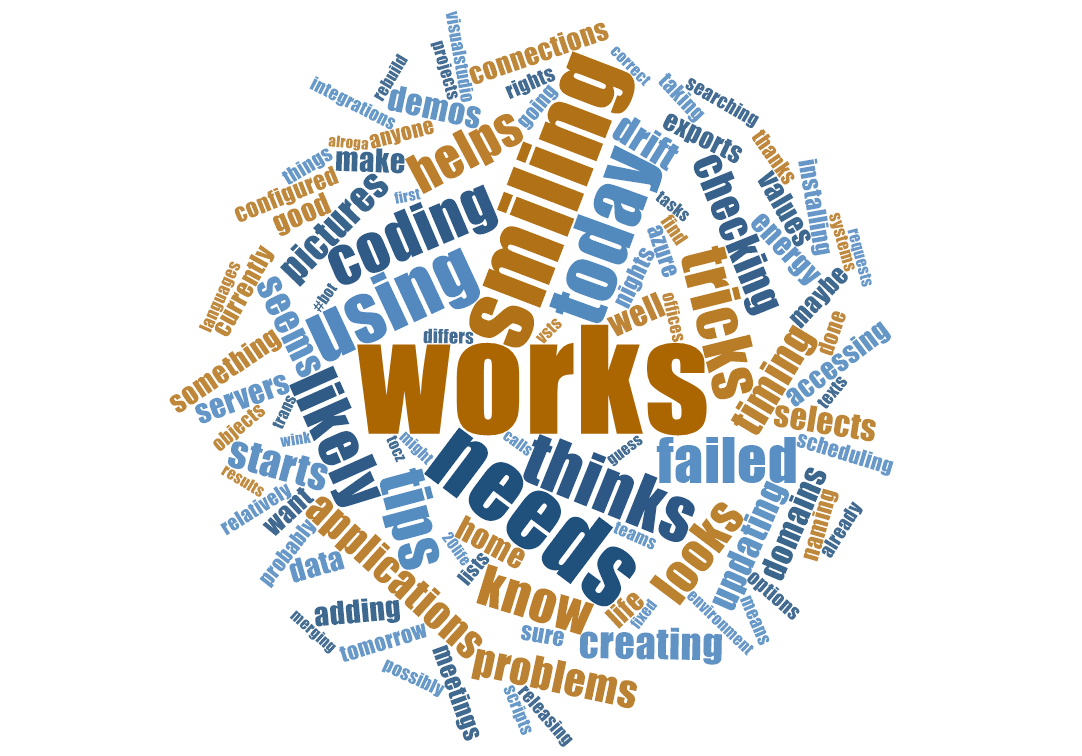
\includegraphics[width=.99\textwidth]{wordcloud.png}
\caption{Word cloud of the first 100 most used words.}\label{fig:wordcloud}
\index{figures}
\end{figure}

\begin{table}
\centering
\caption{The most frequent words} \label{table:word}
\begin{tabular}{cc}
\hline
\textbf{Word} & \textbf{Count} \\ \hline
Works & 2770 \\
Smiling & 1900 \\
Changing & 1216 \\
Needs & 1186 \\
Deploys & 1154 \\
Tricks & 1130 \\
Tips & 1125 \\
Today & 971 \\
Thinks & 916 \\
Issues & 833 \\
\hline
\end{tabular}
\end{table}


 We also did an automatic sentiment analysis of help, general, and backend channels and found the results that are presented in Table \ref{table:sentiment}. Generally, tone of the voices is more neutral, but in the help channel there are more mixed, negative and positive sentiments found compared to the other channels.
 
\begin{table}
\centering
\caption{Sentiment analysis results} \label{table:sentiment}
\begin{tabular}{lc}
\hline
\textbf{Codes} & \textbf{n} \\ \hline
Operations - Mixed&0\\
Operations - Negative&6\\
Operations - Neutral&292\\
Operations - Positive&1\\ \hline
General - Mixed&2 \\
General - Negative&6 \\
General - Neutral&43 \\
General - Positive&8 \\ \hline
Help - Mixed&107\\
Help - Negative&62\\
Help - Neutral&354\\
Help - Positive&32 \\ \hline
Backend - Mixed&4\\
Backend - Negative&8\\
Backend - Neutral&79\\
Backend - Positive&11\\
\hline
\end{tabular}
\end{table}

Also, after coding the logs from three weeks of conversations in general, backend, and operations channels we came to the results presented in Table \ref{table:coded}.

\begin{table}
\centering
\caption{Number of conversation coded in each category in three channels} \label{table:coded}
\begin{tabular}{lccc}
\hline
 & \textbf{Backend} & \textbf{General} & \textbf{Operation} \\ \hline
\textbf{General Answer}&50 &50 &10 \\
\textbf{General Informing}&20 &5 &45 \\
\textbf{General Question}&15 &10 &15 \\
\textbf{Technical Answer}&110 &130 &100 \\
\textbf{Technical Informing}&170 &25 & 150\\
\textbf{Technical Question}&125 &60 &115 \\
\textbf{Socializing}&5 &15 &4 \\
\textbf{Emoji}&15 &90 &70 \\
\hline
\end{tabular}
\end{table}

Here in Table \ref{table:coded} we have the number of codes for each category and see that for example the usage of emoji in the general channel is 6 times more than the backend channel. Respectively number of technical questions drops dramatically in the general channel compared to both backend and operations channel. General questions are asked almost the same in all three channels.

We also looked at number of messages sent per hour in backend and frontend channels. Early in the morning, between 8:00 and 9:00 is the busiest time, in which 686 messages are sent. Then between 9:00 and 13:00 the number of messages sent are stable at around 500 messages per hour, and then halves until 14:00. Then suddenly the number of messages drops substantially to around 90 at 15:00 and steadily goes down until 5:00 in the morning that again starts to rise.

\begin{figure}[hbt!]
\centering
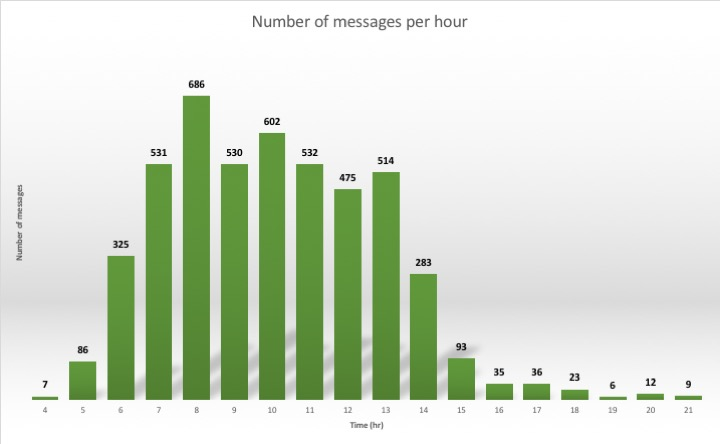
\includegraphics[width=.99\textwidth]{be-fe-messageperhour.jpg}
\caption{Number of messages sent per hour in backend and frontend channels}\label{fig:mph}
\index{figures}
\end{figure}

At the same channels, i.e. backend and frontend, we also looked at the user activity. For privacy reasons the usernames are not converted to real names. Here we see that there are three users who have sent around 500 messages, four other users have also sent more than 200 messages. In total there are 11 users out of 38 who have sent more than 100 messages. 

\begin{figure}[hbt!]
\centering
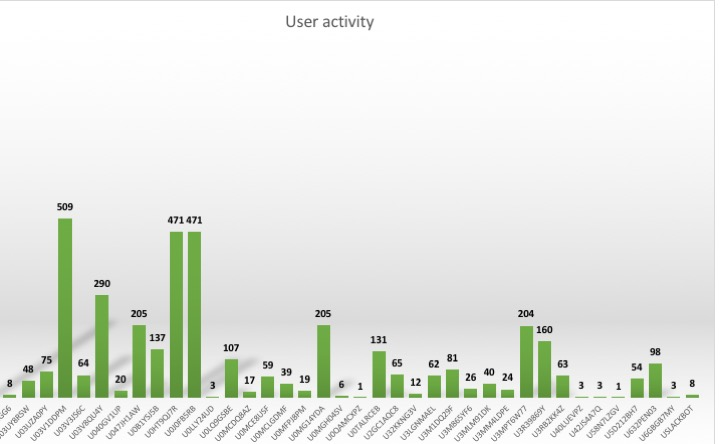
\includegraphics[width=.99\textwidth]{be-fe-useractivity.jpg}
\caption{User activity in backend and frontend channels}\label{fig:useractivity}
\index{figures}
\end{figure}



%\pagebreak
\clearpage
%%%%%%%%%%%%%%%%%%%%%%%%%%%%%%%%%%%%%%%%%%%%%%%%%%%%%%%%%%%%%%%
\section{The survey}
%%%%%%%%%%%%%%%%%%%%%%%%%%%%%%%%%%%%%%%%%%%%%%%%%%%%%%%%%%%%%%%

A total of 172 responses were gathered, of which 97 were completed to the extent that was usable and analyzable. Out of 95 respondents, 87 percent were male (n = 83), and 13 percent female (n = 12) with a mean age of 32 years old (n = 95). Percentage of the respondents who reported that they were working in team was 96 (n = 91), and the proportion of people working in co-located teams (n = 46, 48\%) were slightly less than those who reported working in distributed teams (n = 49, 52\%). The proportion of the team size among the respondents was one-third being in teams of two to five members, one-third in teams with six to eight members and one-third in teams with nine or more members. Table \ref{table:ds} shows the descriptive statistics. 


Among all the respondents, 69\% were software developers, and the rest had roles such as designer, software architect, and manager (Table \ref{table:roles}). The respondents were also asked whether they consider themselves front-end developer, back-end developer or other types of developers. 36\% of all respondents considered themselves as other type of the developers, 26\% considered themselves as back-end developers and 7\% as front-end developers (Table \ref{table:roledetail}). Here there is no meaningful difference between the results gathered through Reddit vs. snowball sampling, except that there were 10\% more back-end developers responding to the survey compared to Reddit users. Looking at the other roles we see that none of the respondents considered themselves as pure testers, which was somehow expected, since the survey was posted in developers forums. 

\begin{figure}[hbt!]
\centering
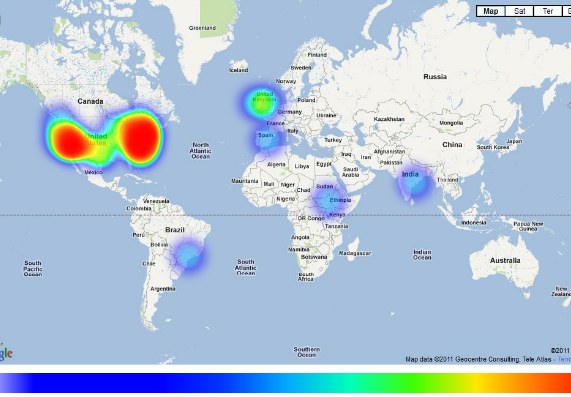
\includegraphics[width=.99\textwidth]{heatmap.png}
\caption{A heatmap of the respondents location}\label{fig:heatmap}
\index{figures}
\end{figure}


\begin{table}
\centering
\caption{Descriptive statistics} \label{table:ds}
\begin{tabular}{lllcc}
\hline
 & \textbf{Unit} & \textbf{n} & \textbf{Mean(M)} & \textbf{Median} \\ \hline
\textbf{Meetings} & Frequency per day & 63 & 2.9 & 3 \\
\textbf{Time in meetings} & Hours per day; \ac{dsm}s included & 48 & 1.4 & 1 \\
\textbf{Team size} & Members including self & 87 & 8.1 & 7 \\
\hline
\end{tabular}
\end{table}



\begin{table}
\centering
\caption{Respondents roles in teams} \label{table:roles}
\begin{tabular}{lcc}
\hline
 & \textbf{n} & \textbf{\%} \\ \hline
\textbf{Developer}&66&69\\
\textbf{Tester}&2&2\\
\textbf{Software Architect}&7&7\\
\textbf{Designer}&9&10\\
\textbf{Manager}&2&2\\
\textbf{Other}&9&10\\
Total&95&100\\
\hline
\end{tabular}
\end{table}


\begin{table}
\centering
\caption{Respondent’s roles in detail} \label{table:roledetail}
\begin{tabular}{lllcc}
\hline
 & \textbf{n(Total)} & \textbf{\%(Total)} & \textbf{\%Reddit} & \textbf{\%Snowballing} \\ \hline
\textbf{Front End Developer}&7&7&8&6 \\
\textbf{Back End Developer}&25&26&23&33 \\
\textbf{Developer}&34&36&35&37 \\
\textbf{Tester}&2&2&0&6 \\
\textbf{Software Architect}&7&7&8&6 \\
\textbf{Designer}&9&10&13&3 \\
\textbf{Manager}&2&2&2&3 \\
\textbf{Other}&9&10&11&6 \\
Total&95&100&100&100 \\
\hline
\end{tabular}
\end{table}

Scrum was the most used development method among the respondents, with almost half of the respondents using it, followed by Kanban which is reported to be used by a quarter of the respondents (Table \ref{table:dm}). The most popular communication media in teams, according to the respondents, were instant messaging (\ac{im}). It is used by more than 90 percent of the respondents. Email follows closely the \ac{im} and is reported to be used by almost 80 percent of the respondents. Face-to-face meetings is the least used communication media by teams, and just 17 percent of our respondents use it (Figure \ref{fig:com-media}).

\begin{table}
\centering
\caption{Development methods used in teams} \label{table:dm}
\begin{tabular}{lcc}
\hline
 & \textbf{n} & \textbf{\%} \\ \hline
\textbf{Scrum}&31&47\\
\textbf{Kanban}&16&24\\
\textbf{Scrumban}&8&12\\
\textbf{XP}&5&8\\
\textbf{Waterfall}&6&9\\
Total&66&100\\
\hline
\end{tabular}
\end{table}



\begin{figure}[hbt!]
\centering
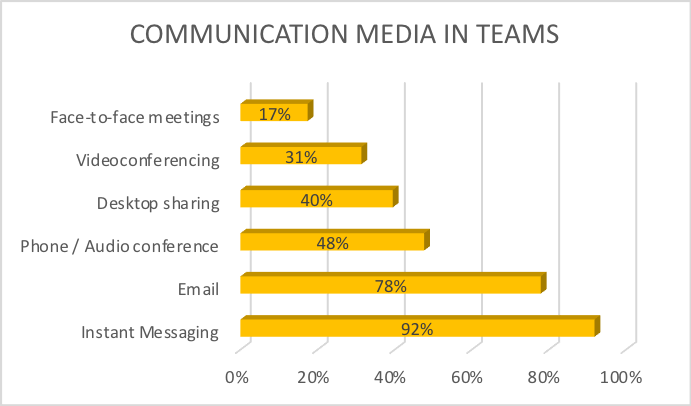
\includegraphics[width=.99\textwidth]{media-in-teams.png}
\caption{Communication media used in teams}\label{fig:com-media}
\index{figures}
\end{figure}



When focusing on specific communication tools, we see that Slack is the biggest winner here, with 59 percent of the respondents using it as their number one means of communication with other team members (Figure \ref{fig:com-tools}). Skype follows Slack by a good distance, and only 38 percent of the respondents use as a communication tool. The third place is occupied by Google Hangout. It is worth mentioning here that Skype and Hangout are more famous for their video calling abilities, while Slack is more text-based, so there would be difficult to compare these tools with each other. In this list Webex, Google Hangout and Skype can be grouped with each other and Slack, HipChat and MS-Teams can be compared to each other (Figure \ref{fig:com-tools}).


\begin{figure}[hbt!]
\centering
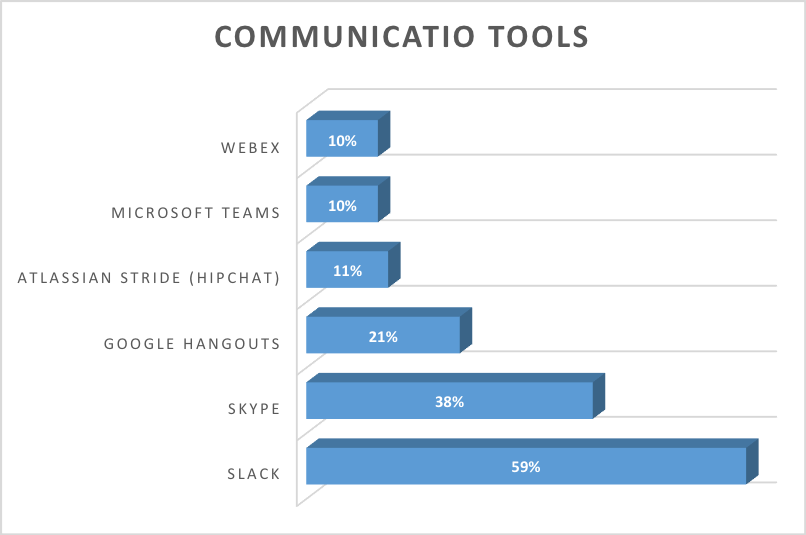
\includegraphics[width=.99\textwidth]{com-tools.png}
\caption{Communication tools used in teams}\label{fig:com-tools}
\index{figures}
\end{figure}

The respondents were also asked what was their biggest challenge while working distributed and almost half of them chose time-zone difference as their biggest challenge. There is no surprise that coordination comes as the second challenge, being chosen by 43 percent of the respondents. Being in different time-zones will immediately affect the coordination between team members. Also, one-third of the respondents chose communication and trust as one of their challenges in their distributed teams (Figure \ref{fig:challenges}).

\begin{figure}[hbt!]
\centering
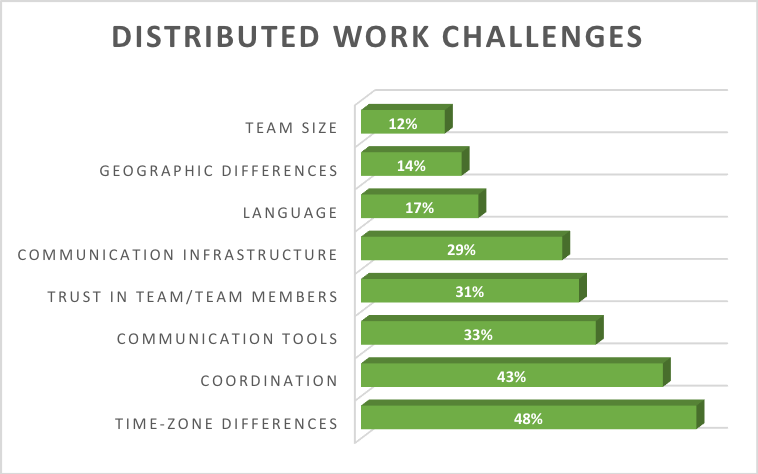
\includegraphics[width=.99\textwidth]{challenges.png}
\caption{Challenges often confronted in distributed teams}\label{fig:challenges}
\index{figures}
\end{figure}

When asked about the frequency of their face-to-face and in-person meetings, one-third of the respondents reported that they never met other team members. 20 percent reported meeting every month, and about one-third chose “other” as the answer to the question (Table \ref{table:f2f}). I also asked the respondents about the purpose of such meetings, and the prominent answer was “status update”, chosen by 27 percent of the respondents. Information sharing and brainstorming were ranked as the second and third purpose of the meetings, chosen respectively by 21 and 15 percent of the respondents (Figure \ref{fig:purpose}). 

\begin{table}
\centering
\caption{Frequency of face-to-face team meetings} \label{table:f2f}
\begin{tabular}{lcc}
\hline
 & \textbf{n} & \textbf{\%} \\ \hline
\textbf{Never}&15&34\\
\textbf{At project kick-off only}&0&0\\
\textbf{Monthly}&9&20\\
\textbf{Every 6 months}&5&11\\
\textbf{Yearly}&2&5\\ 
\textbf{Other}&13&30\\ 
Total&44&100\\
\hline
\end{tabular}
\end{table}


\begin{figure}[hbt!]
\centering
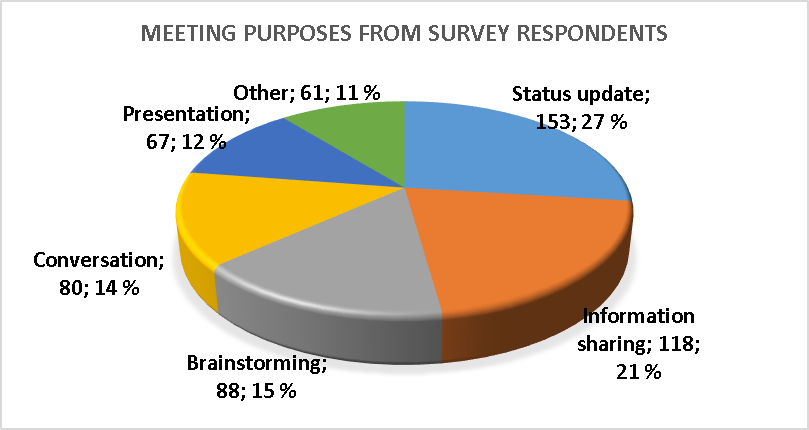
\includegraphics[width=.99\textwidth]{purpose.png}
\caption{Purposes of team meetings}\label{fig:purpose}
\index{figures}
\end{figure}